\documentclass[conference]{IEEEtran}
\usepackage[T1]{fontenc}
\usepackage{graphicx}
\usepackage{amsmath}
\usepackage{booktabs}
\usepackage[hidelinks]{hyperref}
\graphicspath{{../diagrams/}}
% Generated from actual RTL and Yosys outputs.
\newcommand{\GenericCells}{21,192}
\newcommand{\GenericFFs}{9,796}
\newcommand{\ResultRows}{%
Demo & 12 & 7 & 5 & 58.33 & 3.5000 \\
Sequential & 1024 & 768 & 256 & 75.00 & 2.5000 \\
Repeated & 1024 & 1008 & 16 & 98.44 & 1.0938 \\
Random & 1024 & 233 & 791 & 22.75 & 5.6348 \\
Conflict & 1024 & 0 & 1024 & 0.00 & 7.0000 \\
}

\newcommand{\TeamNames}{Navprabhat Singh (Enrollment No. 2401010293)\\ Samarth Khera (Enrollment No. 2401010407)\\ Pratham Malhotra (Enrollment No. 2401010343)\\ Shivansh Tiwari (Enrollment No. 2401020108)\\ Tattva Rajput (Enrollment No. 2401010478)}
\newcommand{\TeamInstitution}{DEPARTMENT NAME PENDING\\COLLEGE NAME PENDING}


\title{Design and Trace-Based Evaluation of a\\Direct-Mapped Cache Controller: Phase I}
\author{\IEEEauthorblockN{\TeamNames}
\IEEEauthorblockA{\TeamInstitution\\Undergraduate project: Phase I prototype}}

\begin{document}
\maketitle
\begin{abstract}
This project implements a synthesizable, blocking direct-mapped cache and
evaluates its behavior using reproducible memory-access traces. The Phase I
prototype has 1 KiB of data capacity, 16-byte lines and 32-bit byte addresses.
It integrates separate data, tag and valid storage with a four-state controller
and an atomic line-refill interface. A self-checking testbench validates reads,
replacement, reset, response backpressure and hit/miss accounting against an
independent software model. Sequential, repeated, seeded random and deliberately
conflicting workloads each contain 1,024 accesses. Their measured hit rates are
75.00\%, 98.44\%, 22.75\% and 0.00\%, respectively. With the supplied memory
model, a hit takes one cycle and a miss seven cycles, giving sequential average
memory access time of 2.5 cycles. Generic logic synthesis provides structural
evidence of implementability. The prototype establishes a read-only baseline
for later write-policy and device-specific extensions.
\end{abstract}
\begin{IEEEkeywords}
direct-mapped cache, Verilog, memory hierarchy, locality, finite-state machine,
cache hit rate, average memory access time
\end{IEEEkeywords}

\section{Introduction and Phase I Objectives}
The project studies cache lookup and refill and relates memory-access patterns
to observable performance. A small direct-mapped organization makes every
placement decision deterministic and permits inspection of the tag, index,
offset and valid state. Phase I aims to produce an executable prototype, an
IEEE-format report and a reproducible demonstration package. The work uses
aligned 32-bit reads, allowing lookup, miss service and statistics to be
validated before adding store policies or a processor interface.

The starting repository contained an address decoder and a preliminary
three-state FSM in commit \texttt{f6fbe40}. This phase preserves that history,
integrates the missing datapath, and extends control to retain a response until
the requester accepts it. The confirmed five-member roster and enrollment
numbers appear in the author block and individual contributions section.
The course title and outstanding personal contribution evidence still need
to be finalized before submission.

\section{Literature Review}
\subsection{Cache Organization and Locality}
Cornell's architecture notes describe locality, direct mapping, valid/tag
lookup and cache filling, together with the standard AMAT expression
\cite{cornell}. These concepts motivate the prototype's separate storage
arrays and its sequential and repeated-access experiments. The former exposes
reuse within a line; the latter exposes reuse of a small working set.

\subsection{Mapping Conflicts}
Jouppi investigates small associative buffers and stream buffers as extensions
to direct-mapped caches \cite{jouppi}. Victim caching retains displaced data
to mitigate mapping conflicts, while stream buffers exploit predictable
access sequences. The present design implements neither extension. Instead,
alternating same-index addresses establishes a measurable conflict baseline
against which such techniques could later be compared.

\subsection{Physical Cache Timing}
Wilton and Jouppi's CACTI work models cache access and cycle time using array
organization and circuit components, including decoders and comparators
\cite{cacti}. It motivates distinguishing architectural cycle counts from
physical implementation timing. This report uses simulated transaction latency
and generic synthesis; it does not infer silicon access time, energy or a
device clock limit from those results.

\subsection{Verification and Synthesis Tools}
Icarus Verilog supplies compilation and simulation of the RTL and testbench
\cite{icarus}. Yosys provides synthesis and structural statistics
\cite{yosys}. Neither tool's successful execution substitutes for testing
on a selected FPGA. The accompanying raw outputs support the limited claims
made in this report.

\section{Proposed Solution}
\subsection{Configuration and Address Derivation}
For cache data capacity $C=1024$ bytes and block size $B=16$ bytes,
\begin{align}
N &= C/B = 64,\\
b &= \log_2 B = 4,\quad i=\log_2 N=6,\\
t &= 32-i-b = 22.
\end{align}
The byte address is divided as follows:
\begin{center}
\begin{tabular}{ccc}
\toprule
Tag & Index & Block offset\\
\midrule
$A[31:10]$ & $A[9:4]$ & $A[3:0]$\\
22 bits & 6 bits & 4 bits\\
\bottomrule
\end{tabular}
\end{center}
Bits $A[3:2]$ select one of four words; $A[1:0]=00$ is required.
The memory request uses block base $\{A[31:4],0000\}$.
Data storage requires 8,192 bits, tags 1,408 bits and validity 64 bits,
giving 9,664 architectural storage bits excluding control and counters.
The cache geometry is fixed in Phase I; memory-model latency is parameterized.

\subsection{Datapath and Interface}
Fig.~\ref{fig:architecture} summarizes the proposed datapath. A CPU request
is accepted only when request-valid and request-ready are both asserted at
a rising clock edge. The latched address drives the decoder, so later changes
on the input cannot corrupt a miss. A hit requires
\begin{equation}
\mathrm{hit} = \mathrm{valid}[\mathrm{index}]\land
(\mathrm{tag}[\mathrm{index}]=\mathrm{requested\ tag}).
\end{equation}
The cache has one outstanding transaction. On a miss, it holds a line-memory
request until the endpoint asserts ready with a complete 128-bit line. Data,
tag and valid are updated together on that transfer. The least significant
32 line bits contain the word at the aligned base address.

\begin{figure}[t]
\centering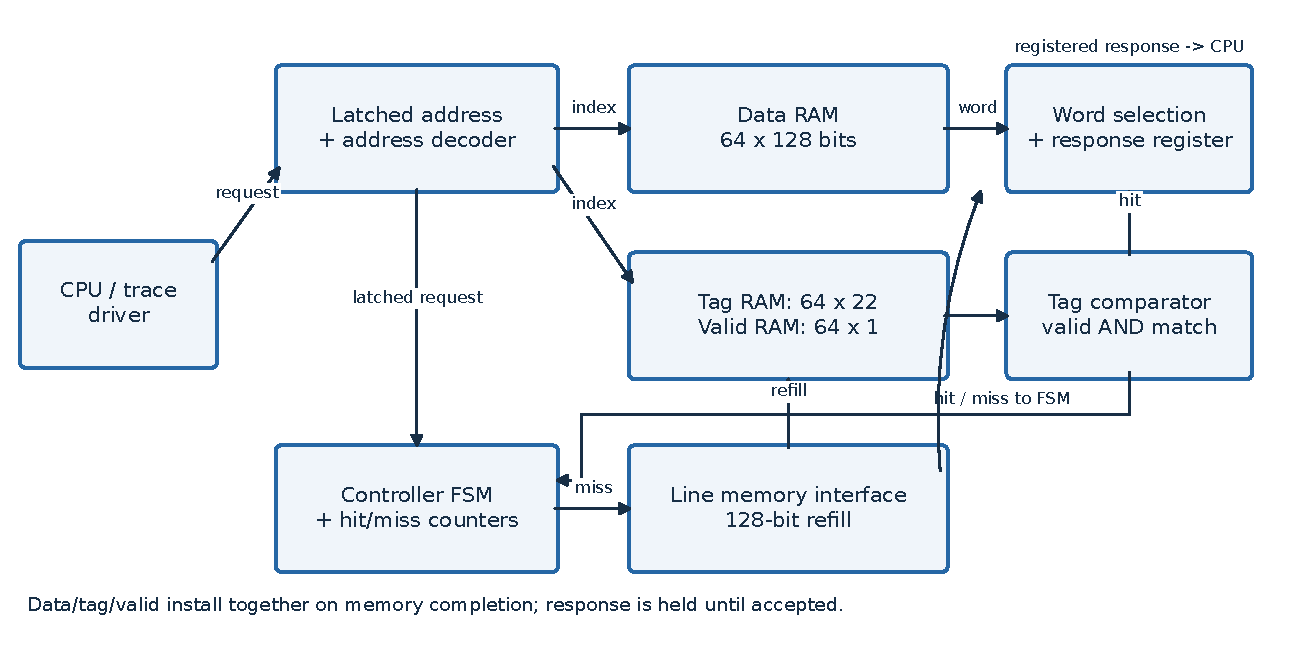
\includegraphics[width=\columnwidth]{architecture.pdf}
\caption{Prototype modules and main datapath connections. Control also gates
atomic installation and holds the registered response until acknowledgment.}
\label{fig:architecture}
\end{figure}

The response includes data, a hit indicator and an error indicator. It stays
stable while response-ready is low. Misaligned addresses return an error and
zero data without allocation or statistics changes. Reset clears every valid
bit and both counters, and aborts the pending response. The memory endpoint
must reset with the cache to cancel an outstanding line request. Data and tag
arrays need no reset because invalid entries cannot produce usable hits.

\subsection{Controller FSM}
The controller has four states (Fig.~\ref{fig:fsm}). IDLE accepts and latches
a request. COMPARE performs one lookup and increments exactly one aligned
access counter. A hit or alignment error proceeds to RESPOND; a miss proceeds
to ALLOCATE. ALLOCATE waits for a whole-line transfer and installs the new
entry. RESPOND retains the result until accepted and then returns to IDLE.
Refill bypasses a second comparison, avoiding double counting.

\begin{figure}[t]
\centering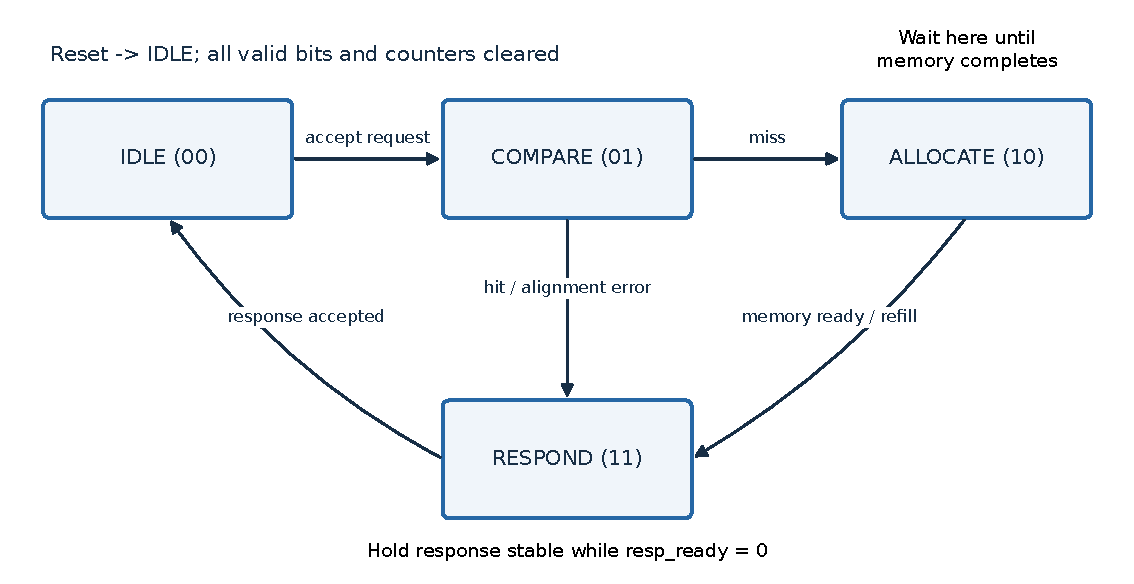
\includegraphics[width=\columnwidth]{fsm.pdf}
\caption{Four-state controller. ALLOCATE and RESPOND wait for their respective
handshakes. Reset returns the controller to IDLE.}
\label{fig:fsm}
\end{figure}

\subsection{Statistics and Timing Convention}
For aligned accesses $A$, hits $H$ and misses $M$,
\begin{equation}
A=H+M,\quad r_h=H/A,\quad r_m=M/A.
\end{equation}
Latency is measured from request acceptance to the first assertion of
response-valid, excluding response backpressure and idle gaps. A hit takes
one cycle. For memory-model latency parameter $L\geq1$, a miss takes $L+2$
cycles, including comparison, request capture and completion. Thus the
additional miss penalty is $L+1$. With $L=5$,
\begin{equation}
\mathrm{AMAT}=T_h+r_m P_m=1+6r_m.
\end{equation}
This follows the standard additional-penalty convention \cite{cornell}.
It describes response latency rather than sustained throughput. At a testbench
period of 10 ns, cycles can be converted to simulation time; this period is
not a measured maximum hardware frequency.

\section{Prototype Implementation and Verification}
The implementation consists of the original \texttt{addr\_decoder.v}, updated
\texttt{cache\_fsm.v}, and separate controller, data, tag, valid and comparator
modules under \texttt{rtl/}. The testbench and memory endpoint reside under
\texttt{tb/}; the latter computes each word as its address XOR
\texttt{0xA5A50000}. This deterministic model covers all address tag bits
without allocating a physical 4 GiB backing array.

A separate Python reference model stores full memory-block numbers at their
mapped slots. It generates expected hit classifications and returned words.
The RTL testbench checks every response, and a post-processing script audits
all output rows independently. Each run also performs 142 directed read
checks, covering cold tag-zero lookup, all four word offsets, all 64 indices
after reset, same-index eviction, high tags, changed inputs while busy,
alignment errors, held responses, exact counters and memory transaction
counts. Additional scenarios reset during allocation and during a pending
response. Timeouts detect a stalled controller.

Each of five workloads is run with memory latency parameters 1, 5 and 9,
giving 15 passing regression runs and 12,324 workload reads. These tests are
directed and trace-based verification; exhaustive formal proof is outside
the current scope. Fig.~\ref{fig:waveform} is rendered from the simulator's
actual VCD output.

An additional 4,096-access stress sequence spans high 32-bit addresses, all
word offsets, reuse and same-index replacement. Both source RTL and the
exported synthesized netlist pass the testbench and match the software oracle;
their complete output CSV files are identical. This checks behavior after
synthesis for the tested sequences and is not an exhaustive equivalence proof.

\begin{figure}[t]
\centering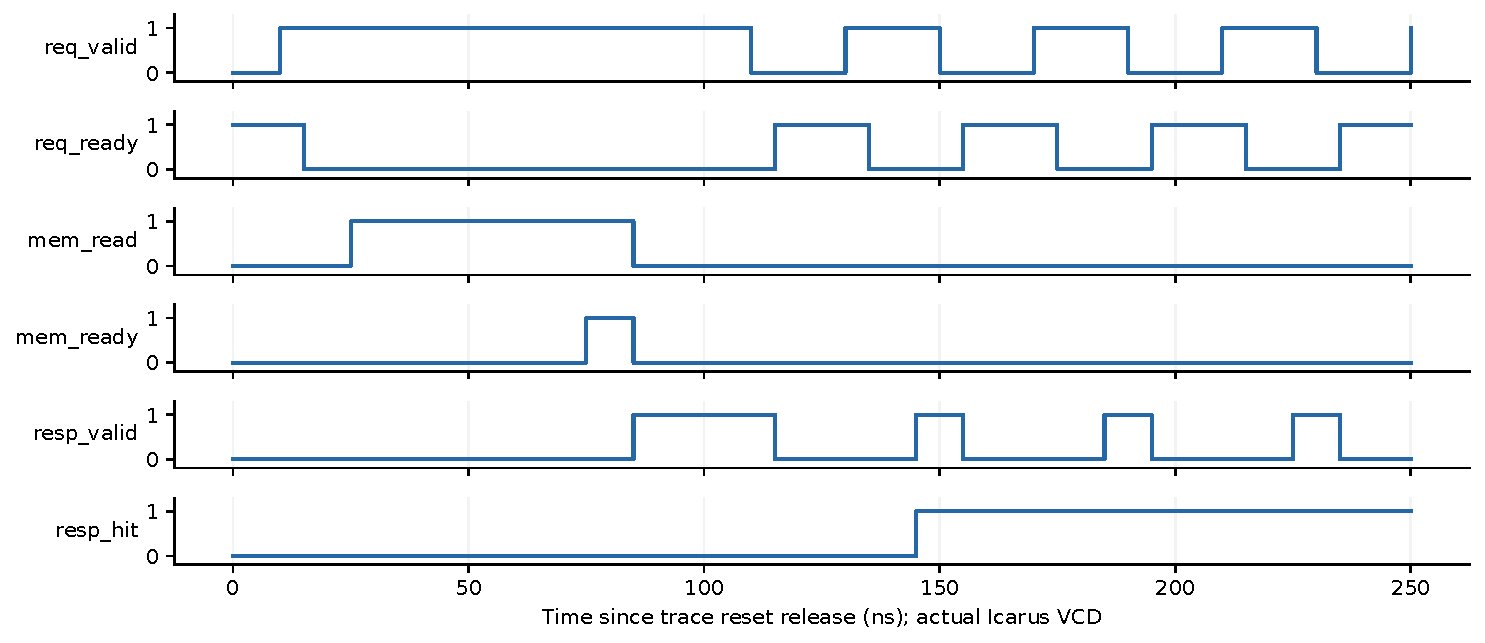
\includegraphics[width=\columnwidth]{waveform.pdf}
\caption{Actual simulator waveform for the beginning of the demo trace,
including a cold miss and later cache hit. Time is relative to trace reset.}
\label{fig:waveform}
\end{figure}

\section{Results and Architectural Analysis}
\subsection{Workloads and Measured Outcomes}
All workloads start from an invalid cache. Sequential reads cover 4 KiB in
word order. Repeated reads traverse a 256-byte set sixteen times. Random reads
use seed 6 over a 4 KiB word-address range. Conflict reads alternate addresses
\texttt{0x00000000} and \texttt{0x00000400}. A short 12-access demonstration
provides an inspectable lookup/replacement example.

\begin{table}[t]
\caption{RTL Measurements at Default Memory Latency}
\label{tab:results}
\centering\footnotesize
\begin{tabular}{lrrrrr}
\toprule
Trace & $A$ & $H$ & $M$ & Hit (\%) & AMAT\\
\midrule
\ResultRows
\bottomrule
\end{tabular}
\end{table}

Table~\ref{tab:results} reports actual RTL output. Sequential traffic has
one initial miss per four-word line, followed by three hits. Repeated traffic
needs only 16 initial fills because its working set fits in the cache.
Random traffic has limited immediate reuse and frequent replacements.
The random result is specific to this trace, not a general prediction.
Conflict traffic continually replaces index zero even though its two-block
working set is small: the first two misses are compulsory and subsequent
misses demonstrate mapping conflicts. Fig.~\ref{fig:results} compares the
observed locality and latency outcomes. These synthetic experiments do not
establish speedup for a complete processor or real application.

\begin{figure}[t]
\centering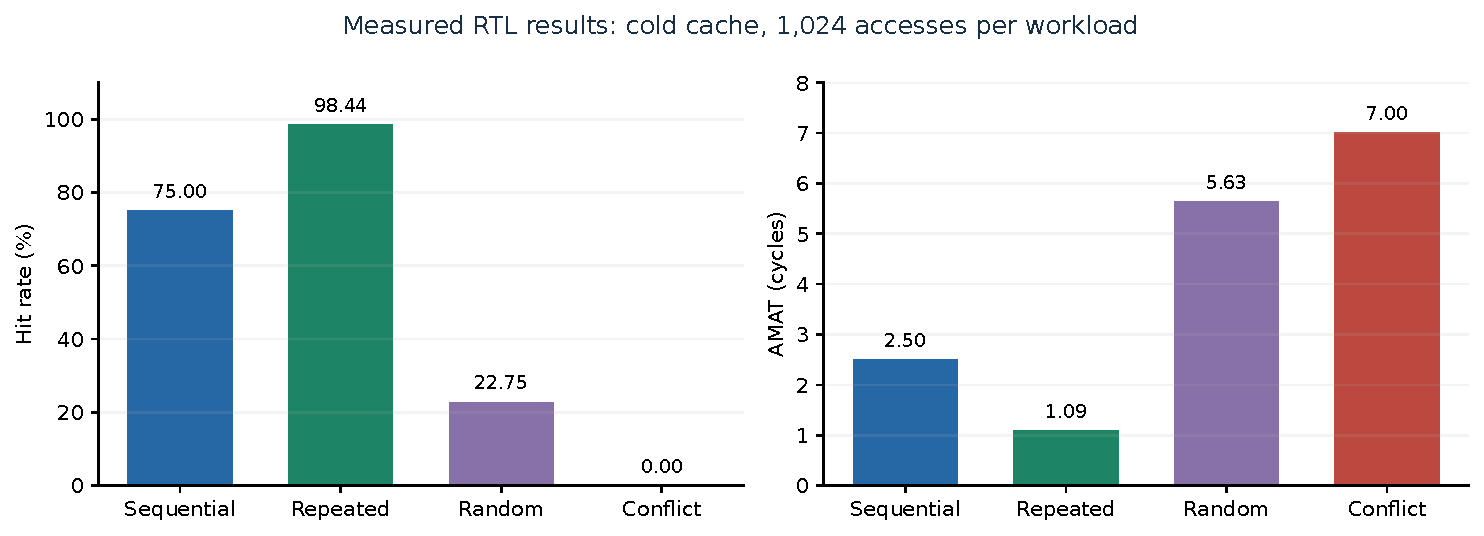
\includegraphics[width=\columnwidth]{results.pdf}
\caption{Hit rate and AMAT for the four 1,024-access workloads.}
\label{fig:results}
\end{figure}

\subsection{AMAT Calculation}
For sequential traffic,
\begin{equation}
\mathrm{AMAT}=1+(256/1024)\times6=2.5\ \mathrm{cycles}.
\end{equation}
For repeated traffic it is $1+(16/1024)\times6=1.09375$ cycles.
For the deliberately conflicting sequence it is seven cycles. In every
workload, the analytical AMAT agrees with the measured mean of individual
request-to-response latencies. This consistency also guards against counting
the seven-cycle total miss latency as an additional penalty.

\subsection{Synthesis Evidence}
Yosys generic synthesis completes with \GenericCells{} leaf logic cells,
including \GenericFFs{} flip-flop cells. The count excludes six hierarchy
instances in the aggregate statistic. Before mapping, two memory cells
represent data and tag arrays; valid bits are registers. Structural
\texttt{check -assert} passes before and after synthesis. The testbench and
backing-memory model are excluded. Raw logs and machine-readable statistics
are included under \texttt{results/}.

The generic flow maps asynchronous-read arrays to registers and multiplexers.
These results are not FPGA LUT counts, physical area, power or timing closure.
A target FPGA, suitable synchronous-memory adaptation, constraints and vendor
flow are necessary before reporting BRAM use or maximum clock frequency.

\section{Individual Contributions}
The original commit attributes the decoder and initial FSM to Samarth Khera's
GitHub account. The new integrated prototype, regression framework and report
were prepared with AI assistance. Proposed responsibilities below must be
replaced with completed, truthful individual work and corresponding commit
evidence. Listing a role alone does not establish a contribution.

\noindent\textbf{Samarth (full name pending) (PENDING).} Original addr\_decoder.v and cache\_fsm.v in commit f6fbe40; subsequent integration is assisted work. Proposed responsibility: Address decoder and controller FSM.

\noindent\textbf{Tattva (full name pending) (PENDING).} Listed in original README; individual implementation contribution not yet evidenced. Proposed responsibility: Data, tag and valid storage review.

\noindent\textbf{MEMBER 3 NAME PENDING (PENDING).} Pending a real member contribution. Proposed responsibility: Integration and memory protocol review.

\noindent\textbf{MEMBER 4 NAME PENDING (PENDING).} Pending a real member contribution. Proposed responsibility: Testbench, trace and result validation.

\noindent\textbf{MEMBER 5 NAME PENDING (PENDING).} Pending a real member contribution. Proposed responsibility: Report, video and reproducibility review.


\section{Phase I Delivery Status and Future Work}
The package includes RTL, self-checking simulation, representative traces,
measured hit/miss and AMAT results, generic synthesis evidence, diagrams,
this report, and a timed five-speaker recording script. A captioned draft
walkthrough includes all five confirmed names and enrollment numbers.
The course title, outstanding individual contribution records, and a hosted
video featuring all five introductions remain submission tasks. Their pending status is recorded in
the repository. Actual GitHub publication and form submission should be
verified separately from local build success.

Later technical phases can add writes and an explicit write policy, evaluate
alternate geometries, and adapt the memory interface for a selected FPGA.
The current prototype intentionally establishes a validated read baseline.

\begin{thebibliography}{00}
\bibitem{cornell} Cornell University, ``Caches,'' CS 3410 course notes,
Spring 2025. [Online]. Available:
\url{https://www.cs.cornell.edu/courses/cs3410/2025sp/notes/caches.html}
\bibitem{jouppi} N. P. Jouppi, ``Improving direct-mapped cache performance
by the addition of a small fully-associative cache and prefetch buffers,''
in \emph{Proc. 17th Annual Int. Symp. Computer Architecture}, 1990,
pp. 364--373, doi: 10.1109/ISCA.1990.134547.
\bibitem{cacti} S. J. E. Wilton and N. P. Jouppi, ``CACTI: An enhanced
cache access and cycle time model,'' \emph{IEEE J. Solid-State Circuits},
vol. 31, no. 5, pp. 677--688, May 1996, doi: 10.1109/4.509850.
\bibitem{icarus} Icarus Verilog contributors, ``Icarus Verilog.'' [Online].
Available: \url{https://github.com/steveicarus/iverilog}
\bibitem{yosys} YosysHQ, ``Generic synthesis script,'' \emph{Yosys
Documentation}. [Online]. Available:
\url{https://yosyshq.readthedocs.io/projects/yosys/en/latest/cmd/index_techlibs_common.html}
\end{thebibliography}
\end{document}
